\chapter{Introduction}
\section{Motivation}

%TODO: Make this prettier
\begin{figure}[ht!]
  \centering
    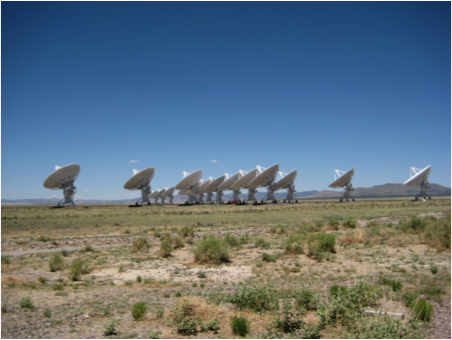
\includegraphics[width=0.49\textwidth]{Images/C1/vla.png}
    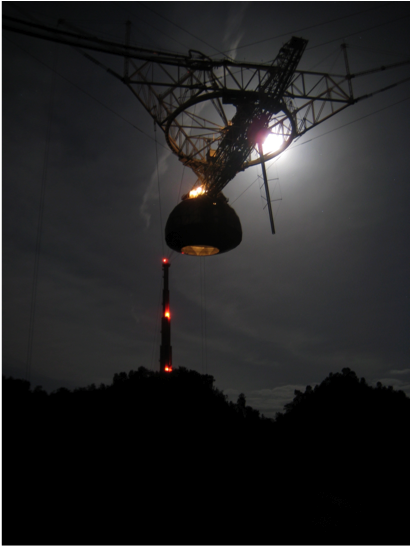
\includegraphics[width=0.49\textwidth]{Images/C1/arecibo.png}
    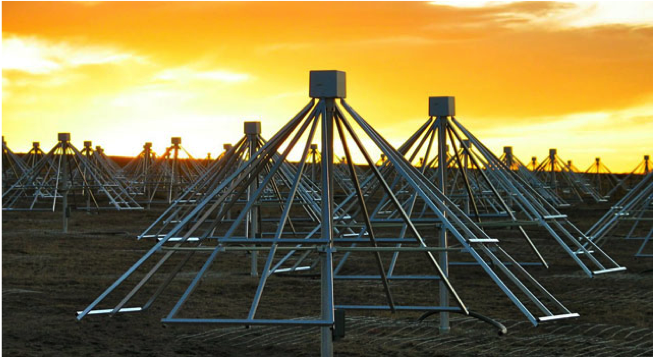
\includegraphics[width=0.49\textwidth]{Images/C1/paper.png}
  \caption{TODO Telescopes}
  \label{fig: C1/telescopes}
\end{figure}


%TODO: Make this prettier, maybe add a graphic
\begin{figure}[ht!]
  \centering
    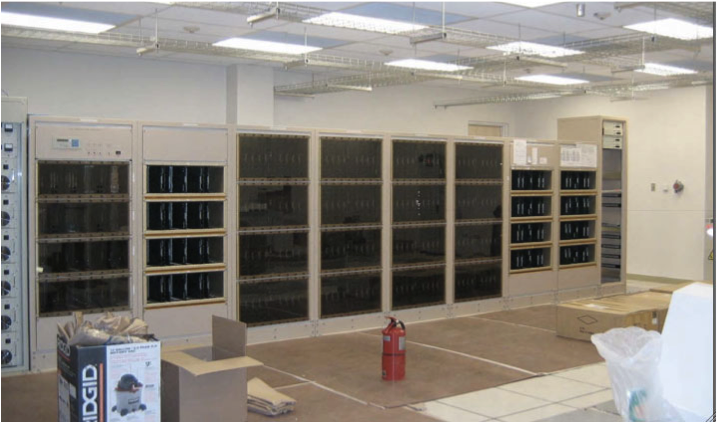
\includegraphics[width=0.49\textwidth]{Images/C1/alma_correlator.png}
    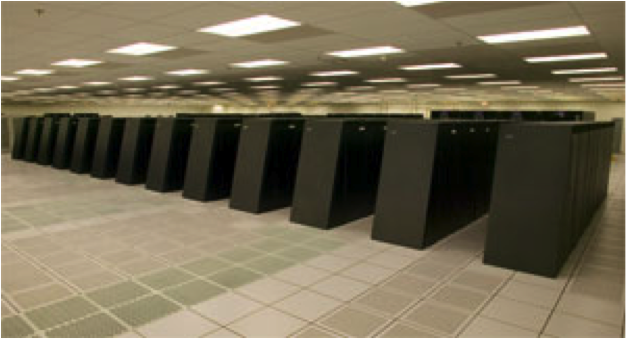
\includegraphics[width=0.49\textwidth]{Images/C1/blue_gene.png}
    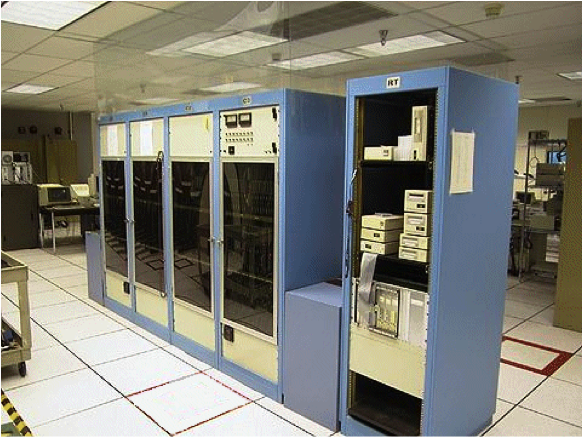
\includegraphics[width=0.49\textwidth]{Images/C1/vla_correlator.png}
  \caption{TODO Building large systems}
  \label{fig: C1/largesystems}
\end{figure}



\begin{figure}[ht!]
  \centering
    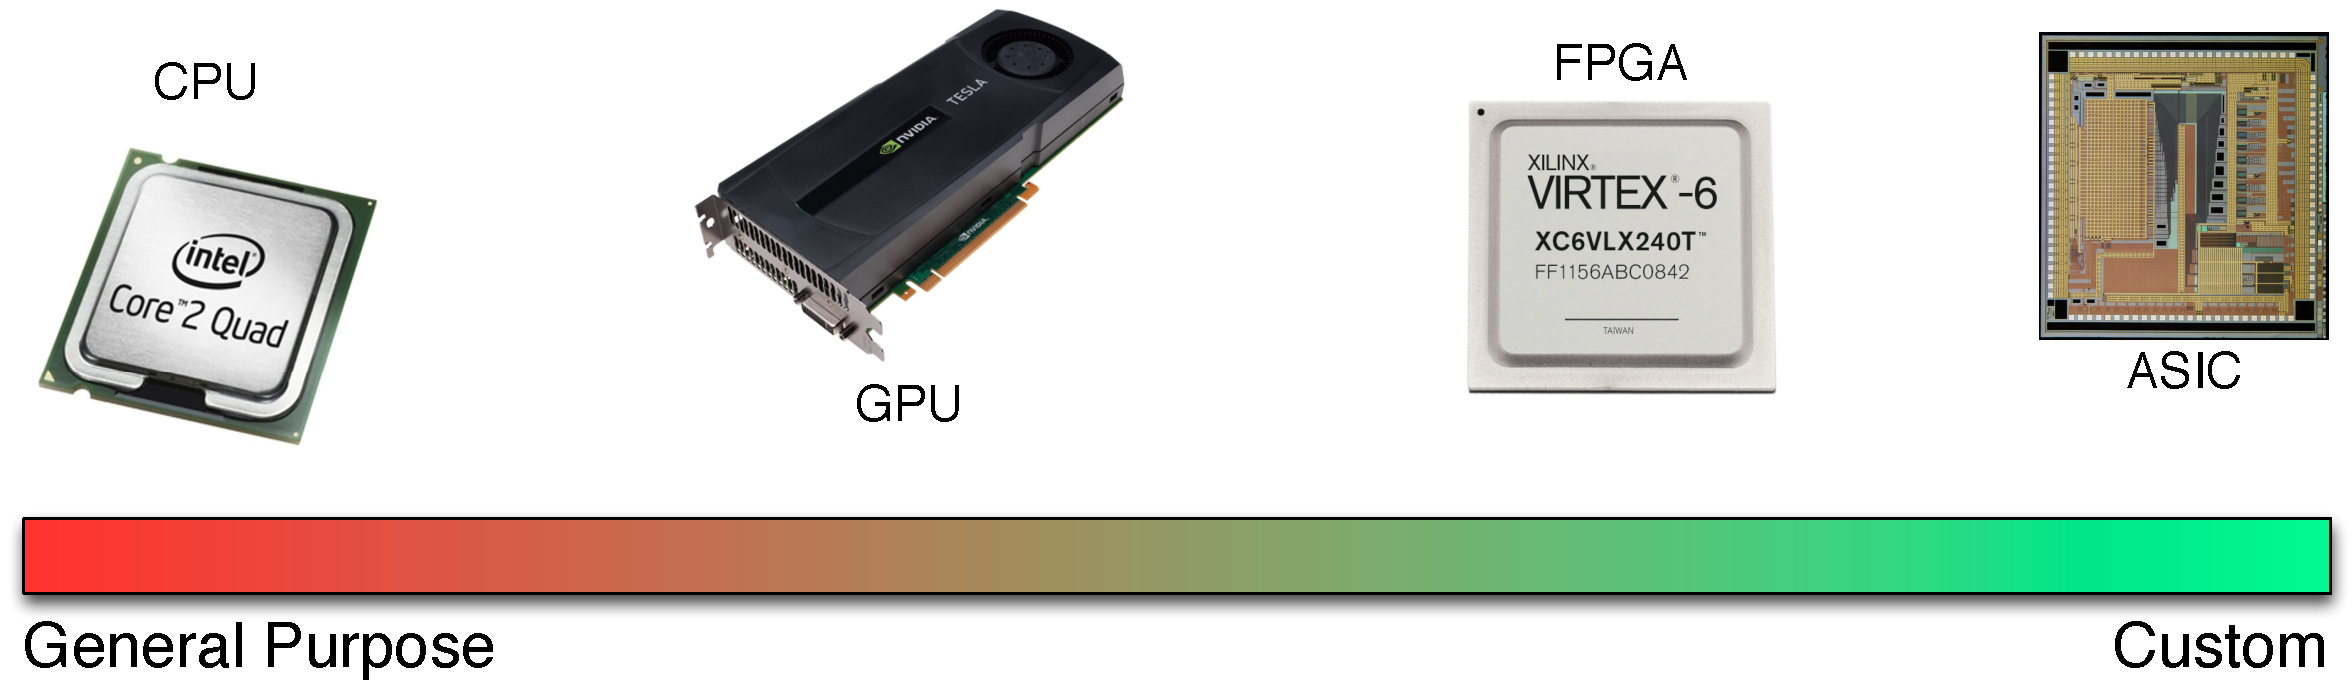
\includegraphics[width=\textwidth]{Images/C1/design_space.pdf}
  \caption{TODO}
  \label{fig: C1/design_space.pdf}
\end{figure}

Increasing

Design time

Design complexity

Performance

Cost (in low volume)

Decreasing

Power (watts)

Flexibility




%Assessing tradeoffs
%3 GHz bandwidth
%100-200 MHz bandwidth
%Fixed point
%Floating point
%Streaming designs
%Conditional/Iterative programming
%Difficult to program (HDL)
%Easy to program (CUDA)
%Difficult to achieve peak performance
%Difficult to achieve peak performance
%$$
%$
%Lots of available IO
%Limited IO

%Traditional instrument design
%Traditionally observatories build custom instruments
%High cost due to custom designed 
%boards
%backplanes
%chips 
%protocols
%software
%Development takes 5 to 10 years
%Hardware is out of date by the time it�s released
%Difficult to upgrade/modify without a redesign



